%!TEX root = ../../beamer.tex
\begin{frame}
Birth-death process \hfill \cite{Erban2007}
{\scriptsize
\begin{align*}
A \xrightarrow{k_1} \varnothing & \hskip 1cm \varnothing \xrightarrow{k_2} A\\
\frac{d \langle A \rangle}{dt} &= k_1 \langle A \rangle - k_2 \langle A \rangle
\end{align*}}
%\vspace{1em}
\begin{center}
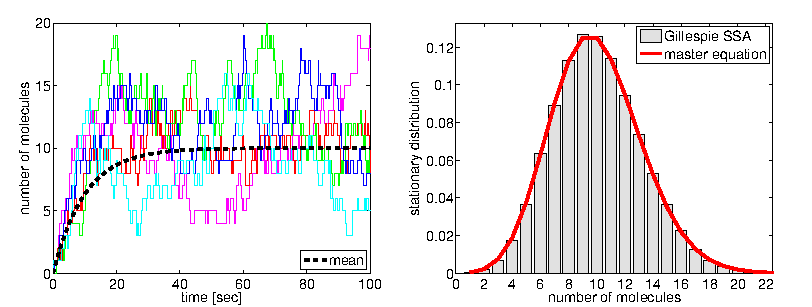
\includegraphics[width=0.9\textwidth]{fig/stochsimbirthdeathprocess.pdf}\\
\end{center}
{\scriptsize
\begin{align*}
\frac{dp_n}{dt}&=k_1(n+1)p_{n+1} - k_1 n p_n + k_2 p_{n-1} - k_2 p_n\\
\phi(n) &= \lim_{t\rightarrow\infty}p_n(t)\\
% 0 &= k_1 \phi(1) - k_2 \phi(0)\\
% 0 &= k_1(n+1)\phi(n+1) - k_1 n \phi(n) + k_2 \phi(n-1) - k_2 \phi(n)\\
\phi(1) &= \frac{k_2}{k_1} \phi(0)\\
\phi(n+1) &= \frac{1}{k_1(n+1)}\left[k_1 n \phi(n) - k_2 \phi(n-1) + k_2 \phi(n) \right]
\end{align*}}
\end{frame}
